\documentclass[12pt, a4paper, oneside]{ctexart}
\usepackage{amsmath, amsthm, amssymb, bm, color, framed, graphicx, hyperref, mathrsfs, float, subfigure}

% multi-column
\usepackage{tasks}
% itemize
\NewTasksEnvironment[label=(\arabic*), label-width=3ex]{exercise}

\everymath{\displaystyle}

\title{\textbf{期中考试(闭卷)}}
\author{U08M11002 Spring 2022; 总分 20 分}
\date{北京时间2022年5月7日19:00-21:00, 教西A101}
\linespread{1}
\definecolor{shadecolor}{RGB}{241, 241, 255}

\newcounter{problemname}
\newenvironment{problem}{\stepcounter{problemname}\par\noindent\textbf{题目\arabic{problemname}. }}{\\\par}
\newenvironment{warning}{\begin{shaded}\par\noindent\textbf{常用傅里叶变换对 / 傅里叶变换定理}}{\end{shaded}\par}

\begin{document}

\maketitle

\begin{warning}
\begin{align*}    
    x(t) = \delta(t) &\overset{\mathcal{F}}\Longleftrightarrow X(j\omega) = 1 \\[10pt]
    x(t) = 1 &\overset{\mathcal{F}}\Longleftrightarrow X(j\omega) = 2\pi\delta(\omega) \\[10pt] 
    x(t) = e^{-\alpha t}U(t) &\overset{\mathcal{F}}\Longleftrightarrow X(j\omega) = \frac{1}{\alpha + j\omega}, \alpha>0 \\[10pt] 
    x(t)=\left\{\begin{matrix} 1, \quad |t|\le T \\ 0, \quad |t|>T \end{matrix}\right. &\overset{\mathcal{F}}\Longleftrightarrow  X(j\omega) = \frac{2\sin(\omega T)}{\omega} \\[10pt]  
    x(t)= \frac{\sin(W t)}{\pi t} &\overset{\mathcal{F}}\Longleftrightarrow  X(j\omega) =\left\{\begin{matrix} 1, \quad |\omega|\le W \\ 0, \quad |\omega|>W \end{matrix}\right.  \\[10pt]
    x_1(t) * x_2(t)  &\overset{\mathcal{F}}\Longleftrightarrow X_1(j\omega)X_2(j\omega)  \\[10pt]
    x_1(t) x_2(t)  &\overset{\mathcal{F}}\Longleftrightarrow \frac{1}{2\pi} X_1(j\omega) * X_2(j\omega)  
\end{align*}

\textbf{傅立叶级数的指数形式}
\begin{align*} 
    f(t) &= \sum_{n=-\infty}^{\infty} F_n e^{jn\Omega t} \\
    F_n &= \frac{1}{T} \int_{-T/2}^{T/2} f(t) e^{-jn\Omega t} dt
\end{align*}

\end{warning}

\newpage
% ----------------------------------
%                第一题
% ----------------------------------
\begin{problem}
(2pts)现有如下图所示的电路。\textbf{请以 P 算子的形式}写出(注意:写成 $p^2$ 前面的系数为 1 的形式):
\begin{figure}[H]
	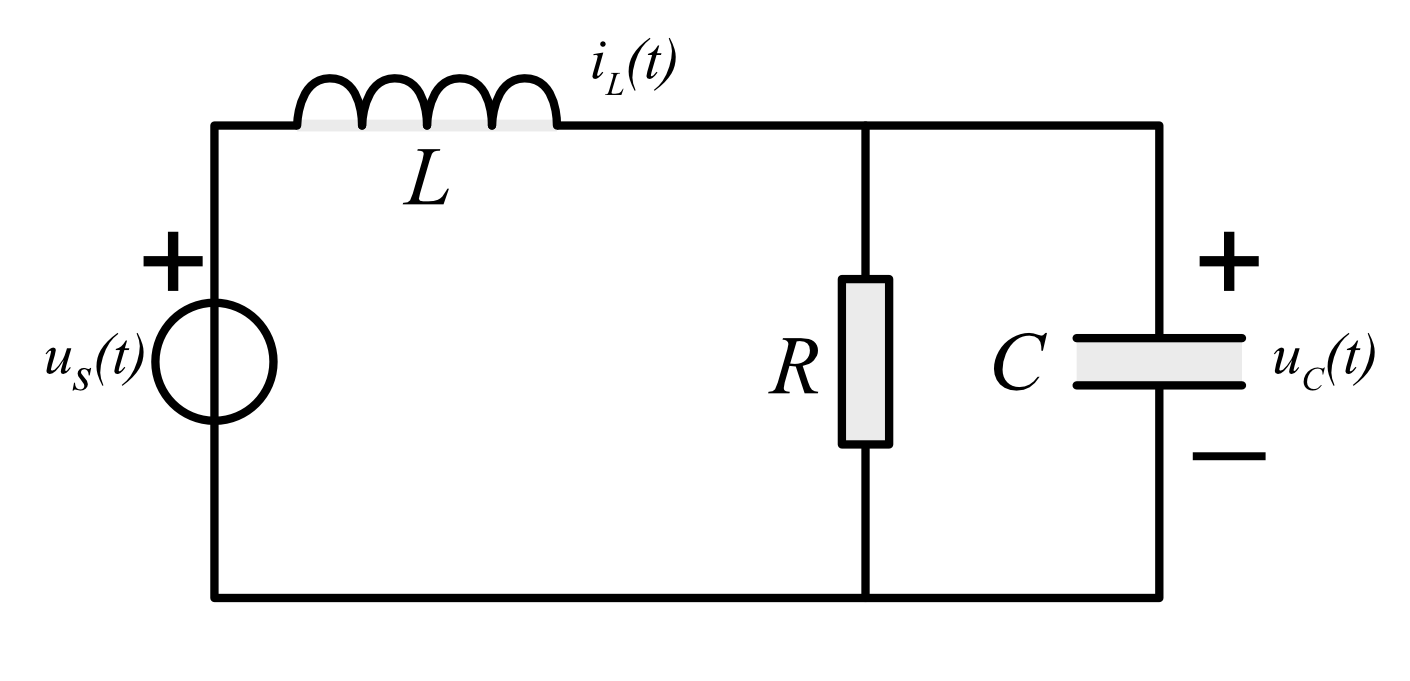
\includegraphics[width=7cm]{assets/hw1img4.png}
	\centering
\end{figure}
\begin{exercise}(1)
	\task (1pt)以 $u_{C}(t)$ 为响应的微分方程;
	\task (1pt)以 $i_{L}(t)$ 为响应的微分方程。
\end{exercise}
\quad
\end{problem}

% ----------------------------------
%                第二题
% ----------------------------------
\begin{problem}
(4pts)已知某 LTI 系统的常微分方程为 $y'(t) + y(t) = f(t)$,
	\begin{exercise}(1)
		\task (1pt)若完全响应为$y(t)=[3e^{-t} + 2e^{-3t}]U(t)$,且 $y(0^-)=3$,求该系统的零输入响应和零状态响应;
		\task (1pt)若$y(0^-)=10$,求系统的零输入响应;
		\task (1pt)若完全响应为$y(t)=[3e^{-t} + 2e^{-3t}]U(t)$,且 $y(0^-)=3$,求$y'(t) + y(t) =f(t-2)$的零状态响应;
		\task (1pt)若完全响应为$y(t)=[3e^{-t} + 2e^{-3t}]U(t)$,且 $y(0^-)=3$,求$y'(t) + y(t) = f'(t) + 3f(t)$的零状态响应。
	\end{exercise}
	\quad
\end{problem}


% ----------------------------------
%                第三题
% ----------------------------------
\begin{problem}
(3pts)求下图\textbf{周期信号}的傅里叶级数,已知 $T = 4\tau$(请给出推导过程,如果直接给结论则不给分)(1pt),并画出频谱幅度图(1pt)。现在,如果$\tau$不变,让周期 T 变成 2T,频谱图会发生什么样的变化(1pt)?
    \begin{figure}[H]
        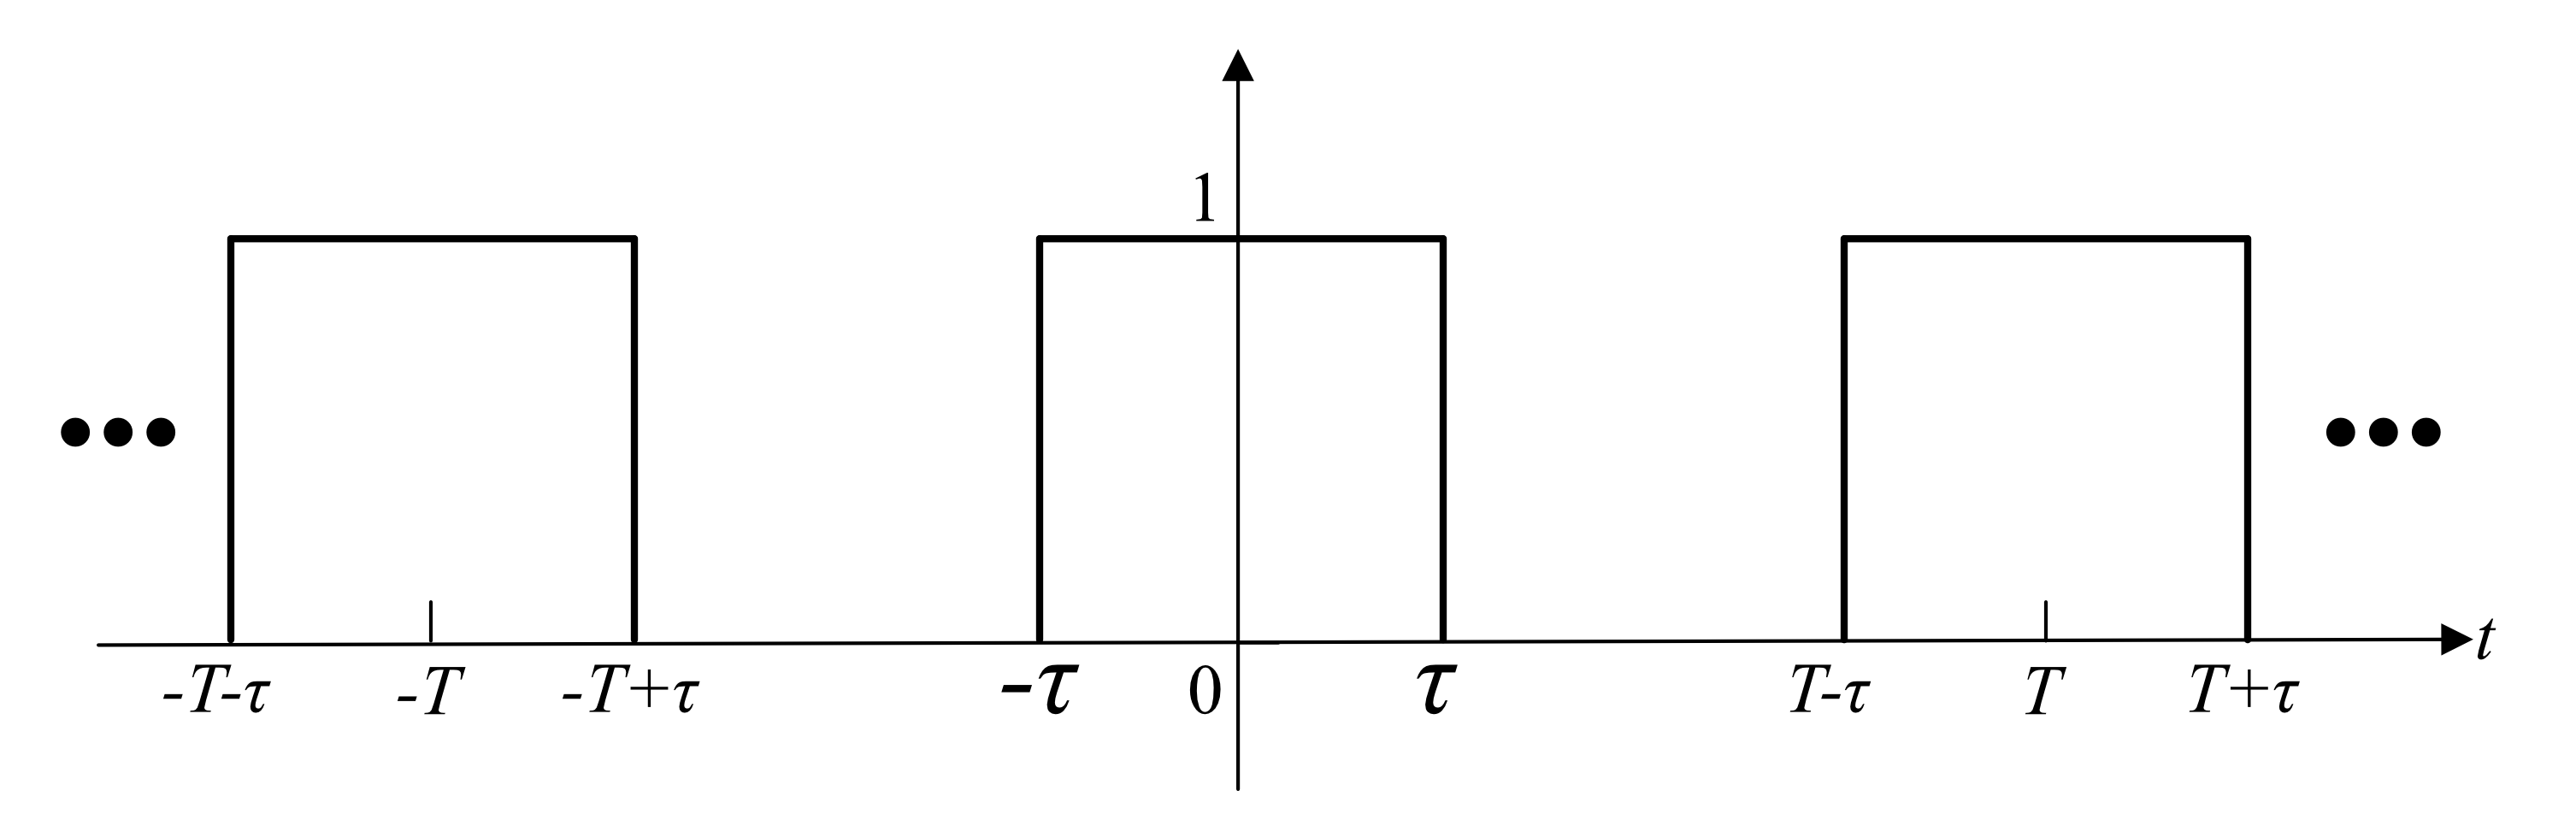
\includegraphics[width=0.8\linewidth]{assets/midtermimg1.png}
        \centering
    \end{figure}
    
\quad
\end{problem}

% ----------------------------------
%                第四题
% ----------------------------------

\begin{problem}
(4pts)已知$f(t) = \Big(\frac{\sin2\pi t}{2\pi t}\Big)^{2}$,$-\infty < t < \infty$,
	\begin{exercise}(1)
		\task (2pts)求$F(jw)$(如果不想列出数学公式,可以画图表示结果。需要给出推理过程。)。
		\task (2pts)求 $\int_{-\infty}^{\infty}f(t) \mathrm{dt}$。
	\end{exercise}	
	\quad
\end{problem}

% ----------------------------------
%                第五题
% ----------------------------------
\begin{problem}
(4pts)描述某线性时不变系统的方程为
	\newline
	$y^{''}(t) + 7y^{'}(t) + 12y(t) = f^{'}(t) + 2f(t)$,试求:
	\begin{exercise}
		\task (2pts)求该系统的冲激响应$h(t)$;
		\task (2pts)若输入$f(t) = 6e^{-t}U(t)$,求系统的零状态响应$y_f(t)$。
	\end{exercise}	
	\quad
\end{problem}

% ----------------------------------
%                第六题
% ----------------------------------
\begin{problem}
(3pts)某一线性系统、输入信号$f(t)$的频谱$F(jw)$ 如下图所示。通过系统$H_1(w)$后便用冲激串$\delta_T(t)$进行抽样,$|H_1(jw)|$的特性如图8(c)所示。
	\begin{exercise}
		\task (1pt)为保证不出现混叠效应,求最低抽样频率$f_s$ (注意:采样频率的单位是 Hz,请注意转换,答案写成角频率不给分);
		\task (1pt)求抽样输出信号$y(t)$的频谱函数(假设采样角频率为$w_s$,采样角频率可以保证不发生频谱混叠);
		\task (1pt)若抽样输出的脉冲调幅信号通过理想信道,为了使接收端能实现无失真地恢复原信号$f(t)$,假设$H_1(jw)$ 在 $[-\omega,\omega]$ 区间是一个线性相位,问接入的系统$H_2(jw)$应具有什么样的特性(请画出$H_2(jw)$的频谱图)。
	\end{exercise}
	\begin{figure}[H]
		\centering
		\subfigure[]{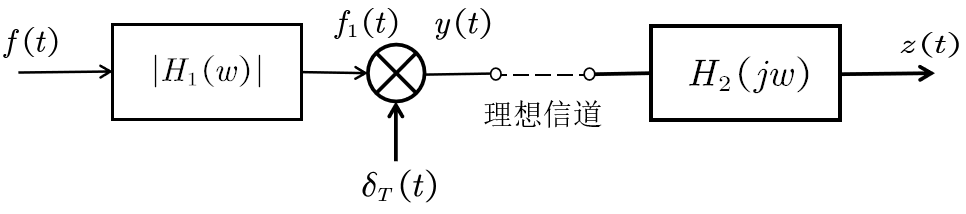
\includegraphics[width=0.9\linewidth]{assets/hw6_9_1.png}}
		\subfigure[]{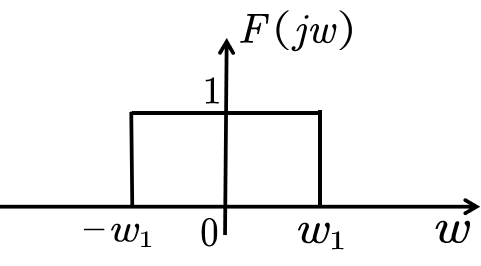
\includegraphics[width=0.39\linewidth]{assets/hw6_9_2.png}}
		\subfigure[]{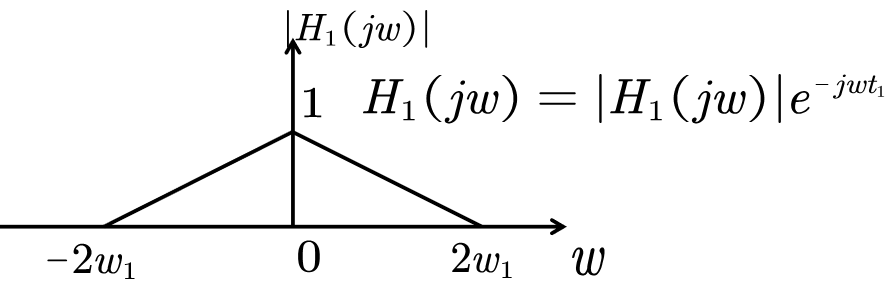
\includegraphics[width=0.59\linewidth]{assets/hw6_9_3.png}}
	\end{figure}
	\quad
\end{problem}

答题纸
\newpage 答题纸
\newpage 答题纸
\newpage 答题纸
\newpage 答题纸

\end{document}